\chapter{\label{c:speedmeter-intro}The \SSMEXPT{}: introduction and technical design}

\section{Concept}
\begin{itemize}
  \item Usual literature review: use 2nd year report, Living Review, Graef et al, etc...
  \item Show Michelson response and noise. This should be radiation pressure dominated below the pole. Relate this to the analytical response equation I used in the controls paper for a Michelson.
  \item Introduce Sagnac speedmeter, showing it has better quantum noise IN ABSENCE OF ASYMMETRIES, and thus better overall sensitivity for equivalent shot noise. DON'T SHOW THE SSM SENSITIVITY HERE.
  \item Use Stefan D's labbook entry for response functions: p5648
  \item Introduce losses to show the degrading effect they have, introducing ``Michelson-like'' sensitivity. The main thing to show here is the effect on the quantum noise when there are asymmetries, like test mass asymmetry. This broadens the peak around the suspension resonance, which introduces the Michelson-like sensitivity.
  \item Mention significance of M8/M9/M10's reflectivity (c.f. loss) which can be expanded later in the controls chapter.
\end{itemize}

As discussed in Section\,\ref{sec:sql}, the \gls{SQL} limits the sensitivity of classical interferometers. Arising from the Heisenberg Uncertainty Principle, the quantum noise present within a classical interferometer\footnote{Note the misnomer: a \emph{classical} interferometer can still be limited by \emph{quantum} noise. The name refers to the readout technique, namely the measurement of classical light power to determine displacement.} It has been known since the time of John von Neumann \note{CITE!} that the use of certain observables can avoid the limit set by the uncertainty principle.

In 1990, Braginsky and Khalili showed that the measurement of momentum, known to be a \emph{quantum non-demolition} (\gls{QND}) observable, offers the ability to surpass the \gls{SQL} in interferometric measurement \cite{Braginsky1990}.





NEW STUFF

The Advanced LIGO gravitational wave observatories \cite{aligo2015} made the first detection of gravitational waves from a binary black hole in 2015 \cite{Abbott2016} at the start of their joint observing run. In the coming years Advanced Virgo \cite{avirgo2015} in Italy and KAGRA \cite{kagra2013} in Japan are expected to join the network, opening up a new window through which to observe the universe. These detectors are, fundamentally, Michelson interferometers with the addition of \FP{} arm cavities and other optical modifications \cite{aligo2015, Abbott2016a} to achieve exquisite sensitivity to motion of the test masses. Using the Local Lorenz gauge, an incident gravitational wave can be pictured as a change in length between the cavity mirrors in each arm of the interferometer. The primary degree of freedom a gravitational wave would excite is the differential mode of the cavity lengths, \LMINUS{}, which can be defined in terms of the position of the end test masses (\glspl{ETM}) $x_{\textrm{A}}^{\textrm{ETM}}$ and $x_{\textrm{B}}^{\textrm{ETM}}$ in cavities A and B, respectively, as:
\begin{equation}
  \label{eq:darm}
  \textrm{\LMINUS{}} = \frac{x_{\textrm{A}}^{\textrm{ETM}} - x_{\textrm{B}}^{\textrm{ETM}}}{2}.
\end{equation}

Quantum noise, the combination of quantum radiation pressure noise at low frequencies and quantum shot noise at high frequencies, restricts the ultimate sensitivity of classical Michelson interferometers at what is termed the \emph{Standard Quantum Limit} (\gls{SQL}) \cite{Braginsky1995}. As quantum noise is expected to limit the sensitivity of the aforementioned \emph{second generation} detectors over a wide frequency band, particular effort is being paid to its reduction in proposals for \emph{third-generation} instruments such as the Einstein Telescope facility \cite{Hild2011} and LIGO Cosmic Explorer \cite{aligoinst2015}.

Reduction of quantum noise below the SQL in a particular optical configuration involves a so-called \emph{quantum non-demolition} (\gls{QND}) measurement \cite{Braginsky1995}: either the use of quantum correlations in the outgoing light or the enhancement of the test mass dynamics by means of light \cite{Chen2011}. Quantum correlations arise naturally between the otherwise uncorrelated sources of quantum noise due to the interaction between the light and the motional degrees of freedom of the interferometer and can be used to effectively avoid radiation pressure noise contributions to the readout signal. This group of methods includes frequency-dependent squeezing \cite{Kimble2001}, variational readout \cite{Kimble2001, Vyatchanin1995, Vyatchanin1996} and speed meters \cite{Braginsky1990, Braginsky2000, Chen2003, Danilishin2004}. The latter approach implies the use of light-mirror interactions to create new test mass dynamics in order to increase their response to the gravitational wave action. This includes so-called ``optical springs'' \cite{Braginsky1999, Buonanno2002, Corbitt2007, Rehbein2008, Gordon2015}, ``optical inertia'' \cite{Khalili2011, Voronchev2012} and ``intracavity schemes'' \cite{Braginsky1997, Khalili2002, Danilishin2006}.
   
The method on which we focus employs an interferometer topology intrinsically sensitive to a QND observable \cite{Danilishin2012}. The measurement of velocity, itself approximately proportional to the QND observable of the free test mass momentum, is one way in which a reduction in quantum radiation pressure noise can be achieved. A proof-of-concept experiment is under way at the University of Glasgow to demonstrate an audio-band reduction of quantum radiation pressure noise in a \SSM{} topology over an equivalent Michelson design \cite{Graef2014}. This topology is being considered as an alternative to the Einstein Telescope's Michelson interferometer design \cite{MuellerEbhardt2009a, Voronchev2015}. The topology under investigation in the proof-of-concept experiment utilises a zero-area Sagnac interferometer with the addition of arm cavities based on the concept presented in ref.\,\cite{Chen2003}. By design, this interferometer produces a signal at the beam splitter's output port proportional to differential arm cavity mirror \emph{velocity}, in contrast to the \emph{displacement}-proportional signal sensed in the Michelson topology.

\subsection{Measurement of speed}

\subsection{Reduced radiation pressure noise over an equivalent \MI{}}

\subsection{\label{sec:bhd-intro}Balanced homodyne detection}
\note{Explain homodyne angle, basic description.}

\section{Implementation}

Some technical challenges in the implementation of the speedmeter are discussed in this chapter. Certain topics involve substantially more scientific endeavour and are thus presented as discrete chapters: the control of the primary degree of freedom of the speedmeter, presented in Chapter X; and a proof-of-principle experiment to demonstrate a new type of actuator, presented in Chapter Y.

\subsection{Experimental design}
\note{Discuss the experiment layout, power, cavity lengths, etc. Introduce the real sensitivity curves here.}

\subsection{Mechanics}
\note{Vacuum system requirements, tanks, optical table, suspensions, seismic noise, etc.}

\subsection{Layout}

\begin{figure}
  \centering
  \includegraphics[width=\columnwidth]{graphics/generated/from-svg/40-speedmeter-layout.pdf}
  \caption[\SSMEXPT{} layout]{\label{fig:ssm-layout}\SSMEXPT{} layout.}
\end{figure}

\subsection{Sensing and control}

\note{Introduce CDS with the Bork reference, as it is required for Chapters 5 and 7}

\subsubsection{Avoidance of ground loops}

One of the main issues faced by experiments involving numerous interfaces between digital and analogue devices is the creation of ground loops. Effectively an antenna.

\note{Avoidance of ground loops, interfacing with CDS, in-vacuum wiring: why it needs careful thought, etc}
\note{Display wiring diagrams in landscape mode, full page}

\note{Generate A4 versions of wiring diagrams for inclusion here.}

\subsubsection{Connectors}
\note{How we avoided plugging the wrong things in, i.e. why we use DB9/DB15/DB25 etc.}
\note{Differential sending - take stuff from HV chapter on CMRR?}

\subsubsection{In-vacuum signalling}
\note{Octopus cables, strain relief housing, etc.}

\begin{figure}
  \centering
  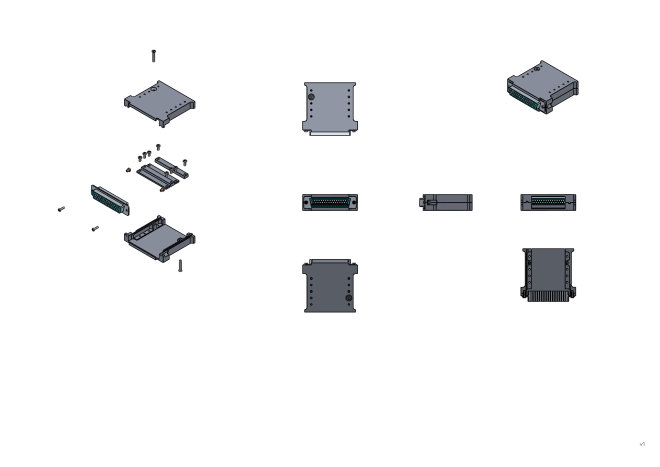
\includegraphics[width=0.75\columnwidth]{graphics/40-db50-housing.png}
  \caption[In-vacuum DB50 octopus cable housing]{In-vacuum DB50 housing for octopus cable.}
  \label{fig:db50-housing}
\end{figure}

\subsubsection{Auxiliary coil drivers}
\note{Put aux coil driver stuff here}
\note{Auxiliary coil driver subrack wiring design / motivation / assembly}
\note{Backplane board design - talk about rationale, show Eagle diagrams, etc.}

\begin{figure}
  \centering
  \includegraphics[width=\columnwidth]{graphics/generated/from-svg/40-auxiliary-octopus-cable.pdf}
  \caption[Auxiliary octopus cable schematic]{\label{fig:aux-octopus-cable-wiring}``Octopus'' cable for breaking out a DB50 connector into DB9 connectors to allow signals to be sent to each of the coils on seven auxiliary suspensions.}
\end{figure}

\begin{figure}
  \centering
  \includegraphics[width=\columnwidth]{graphics/generated/from-svg/40-auxiliary-suspension.pdf}
  \caption[Auxiliary suspension coil schematic]{\label{fig:aux-suspension-wiring}Auxiliary suspension coil schematic.}
\end{figure}

\begin{figure}
  \centering
  \includegraphics[width=\columnwidth]{graphics/generated/from-svg/40-auxiliary-backplane-board.pdf}
  \caption[Auxiliary subrack backplane board schematic]{\label{fig:aux-backplane-schematic}Auxiliary coil driver subrack backplane. Auxiliary coil driver cards can be plugged in to this board, which then maps the signals to a DB50 connector which connects to the vacuum feedthrough. This routes four coil signals (five conductors including ground) per coil driver, for seven coil drivers, to one DB50 connector. This can then be connected to the vacuum system, where the auxiliary octopus cable (see Figure XXX) maps these signals to individual auxiliary suspensions.}
\end{figure}

\begin{figure}
  \centering
  \includegraphics[width=\columnwidth]{graphics/generated/from-svg/40-auxiliary-backplane-interface.pdf}
  \caption[Auxiliary subrack backplane interface]{\label{fig:aux-backplane-interface}Auxiliary coil driver subrack backplane interface.}
\end{figure}

\section{Modelling the sensitivity of the \SSM{}}
\note{Optickle and Finesse models, analytical comparison}